\documentclass{beamer}

% Tema minimalista
\usetheme{default}
\usecolortheme{default}

% Configuración minimalista
\setbeamertemplate{navigation symbols}{}
\setbeamertemplate{footline}[frame number]
\setbeamertemplate{headline}{}

\usepackage[utf8]{inputenc}
\usepackage[spanish]{babel}
\usepackage{lmodern}
\usepackage{graphicx}
\usepackage{booktabs}
\usepackage{amsmath}

% Colores
\definecolor{tecblue}{RGB}{0,56,101}
\setbeamercolor{structure}{fg=tecblue}
\setbeamercolor{title}{fg=tecblue}
\setbeamercolor{frametitle}{fg=tecblue}
\setbeamercolor{block title}{bg=tecblue!20,fg=tecblue}
\setbeamercolor{block body}{bg=tecblue!5}

\title{Análisis Predictivo del Mercado Inmobiliario}
\subtitle{Regresión Lineal Múltiple - Airbnb}
\author{Universidad Tecmilenio}
\date{\today}

\begin{document}

% ============================================
% SLIDE 1: PORTADA
% ============================================
\begin{frame}
  \titlepage
\end{frame}

% ============================================
% SLIDE 2: LIMPIEZA DE DATOS
% ============================================
\begin{frame}{1. Limpieza de Datos}
  \framesubtitle{Preparación del dataset para análisis}
  
  \begin{block}{Proceso de Limpieza}
    \begin{enumerate}
      \item \textbf{Imputación:} Valores faltantes con mediana (bathrooms, bedrooms, beds)
      \item \textbf{Eliminación:} 14 columnas irrelevantes (IDs, URLs, fechas)
      \item \textbf{Outliers:} Método IQR en beds, accommodates, log\_price
    \end{enumerate}
  \end{block}
  
  \vspace{0.3cm}
  
  \begin{center}
    \begin{tabular}{lrr}
      \toprule
      \textbf{Métrica} & \textbf{Original} & \textbf{Limpio} \\
      \midrule
      Filas & 74,111 & 66,752 \\
      Columnas & 29 & 14 \\
      Valores faltantes & 83,752 & 0 \\
      \bottomrule
    \end{tabular}
  \end{center}
  
  \begin{alertblock}{Resultado}
    Dataset limpio: \alert{66,752 observaciones} × \alert{14 variables}
  \end{alertblock}
\end{frame}

% ============================================
% SLIDE 3: IDENTIFICACIÓN DE VARIABLES
% ============================================
\begin{frame}{2. Identificación de Variables}
  
  \begin{block}{Variable Dependiente (Y)}
    \texttt{log\_price} — Logaritmo natural del precio de la propiedad
  \end{block}
  
  \vspace{0.3cm}
  
  \begin{block}{Variables Independientes Candidatas (X)}
    \textbf{Numéricas / Binarias:}
    \begin{itemize}
      \item accommodates, bedrooms, bathrooms, beds
      \item amenities\_count, cleaning\_fee, instant\_bookable
    \end{itemize}
    
    \textbf{Categóricas:}
    \begin{itemize}
      \item room\_type (Entire home, Private room, Shared room)
      \item property\_type, bed\_type, neighbourhood
      \item city, cancellation\_policy, zipcode
    \end{itemize}
  \end{block}
  
  \vspace{0.2cm}
  
  \begin{center}
    \textbf{Total:} 7 numéricas + 7 categóricas = 14 variables candidatas
  \end{center}
\end{frame}

% ============================================
% SLIDE 4: SELECCIÓN DE CARACTERÍSTICAS
% ============================================
\begin{frame}{3. Selección de Características}
  \framesubtitle{Análisis de multicolinealidad (VIF) y correlación}
  
  \begin{columns}
    \column{.5\textwidth}
      \textbf{Variables EXCLUIDAS:}
      \begin{itemize}
        \item[\alert{$\times$}] \texttt{beds} \\
        VIF = 14.89 (crítico)
        \item[\alert{$\times$}] \texttt{bathrooms, bedrooms} \\
        Colinealidad moderada y ruido
        \item[\alert{$\times$}] \texttt{zipcode} \\
        Redundante y de altísima cardinalidad
      \end{itemize}
    
    \column{.5\textwidth}
      \textbf{Variables INCLUIDAS:}
      \begin{itemize}
        \item[\textcolor{green}{$\checkmark$}] \texttt{accommodates} \\
        Predictor principal
        \item[\textcolor{green}{$\checkmark$}] \texttt{amenities\_count, cleaning\_fee, instant\_bookable} \\
        Nuevas variables añadidas
        \item[\textcolor{green}{$\checkmark$}] \texttt{room\_type, property\_type, bed\_type, city, cancellation\_policy} \\
        Variables dummy relevantes
        \item[\textcolor{green}{$\checkmark$}] \texttt{neighbourhood} \\
        (609 variables dummy)
      \end{itemize}
      
      \vspace{0.3cm}
      
      \textbf{Total: >650 predictores}
  \end{columns}
  
  \vspace{0.3cm}
  
  \begin{alertblock}{Criterio}
    VIF $<$ 5 y relevancia técnica en el modelo
  \end{alertblock}
\end{frame}

% ============================================
% SLIDE 5: ANÁLISIS DE CORRELACIÓN
% ============================================
\begin{frame}{4. Análisis de Correlación}
  \framesubtitle{Pairplot y matriz de correlación}
  
  \begin{center}
    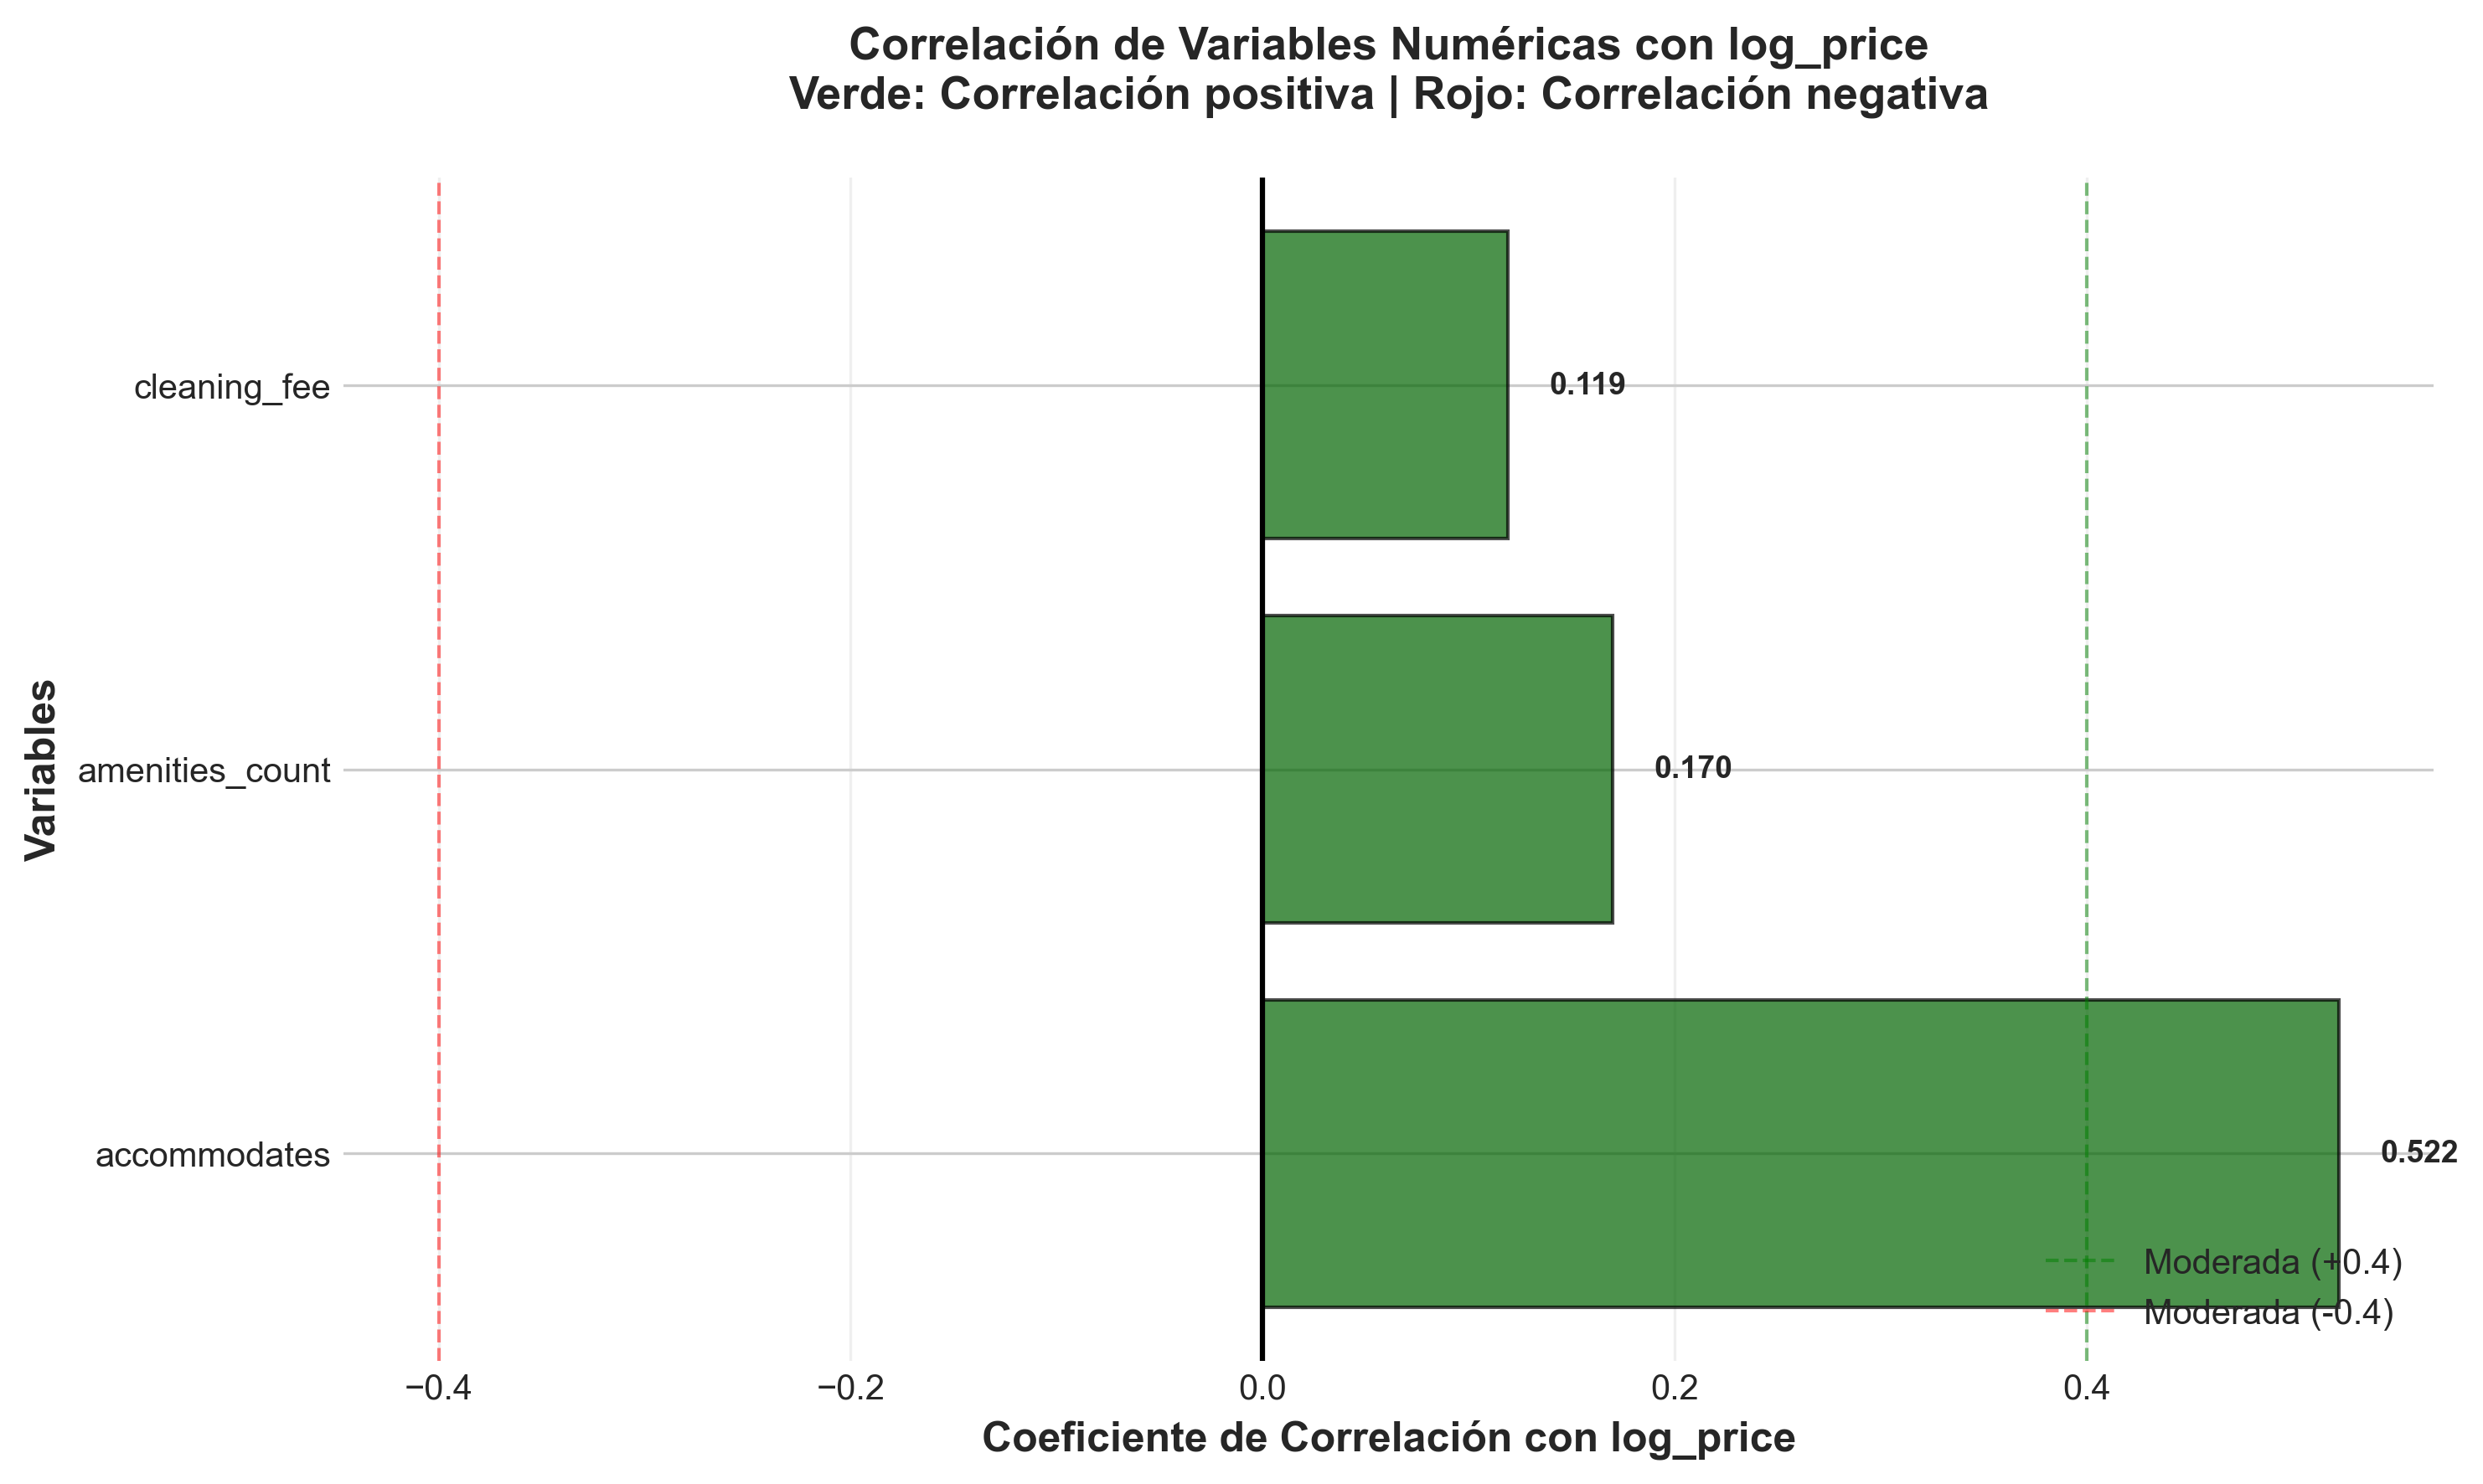
\includegraphics[width=0.95\textwidth]{../Visualizaciones/proyectoFinal/10_correlaciones_log_price_barras.png}
  \end{center}
  
  \vspace{-0.2cm}
  
  \begin{itemize}
    \item \textbf{accommodates:} +0.522 (predictor principal)
    \item \textbf{bedrooms:} +0.293 (excluida por colinealidad)
    \item \textbf{bathrooms:} +0.155 (excluida por colinealidad)
  \end{itemize}
\end{frame}

% ============================================
% SLIDE 6: DIVISIÓN TRAIN-TEST
% ============================================
\begin{frame}{5. Grupos de Entrenamiento y Prueba}
  
  \begin{center}
    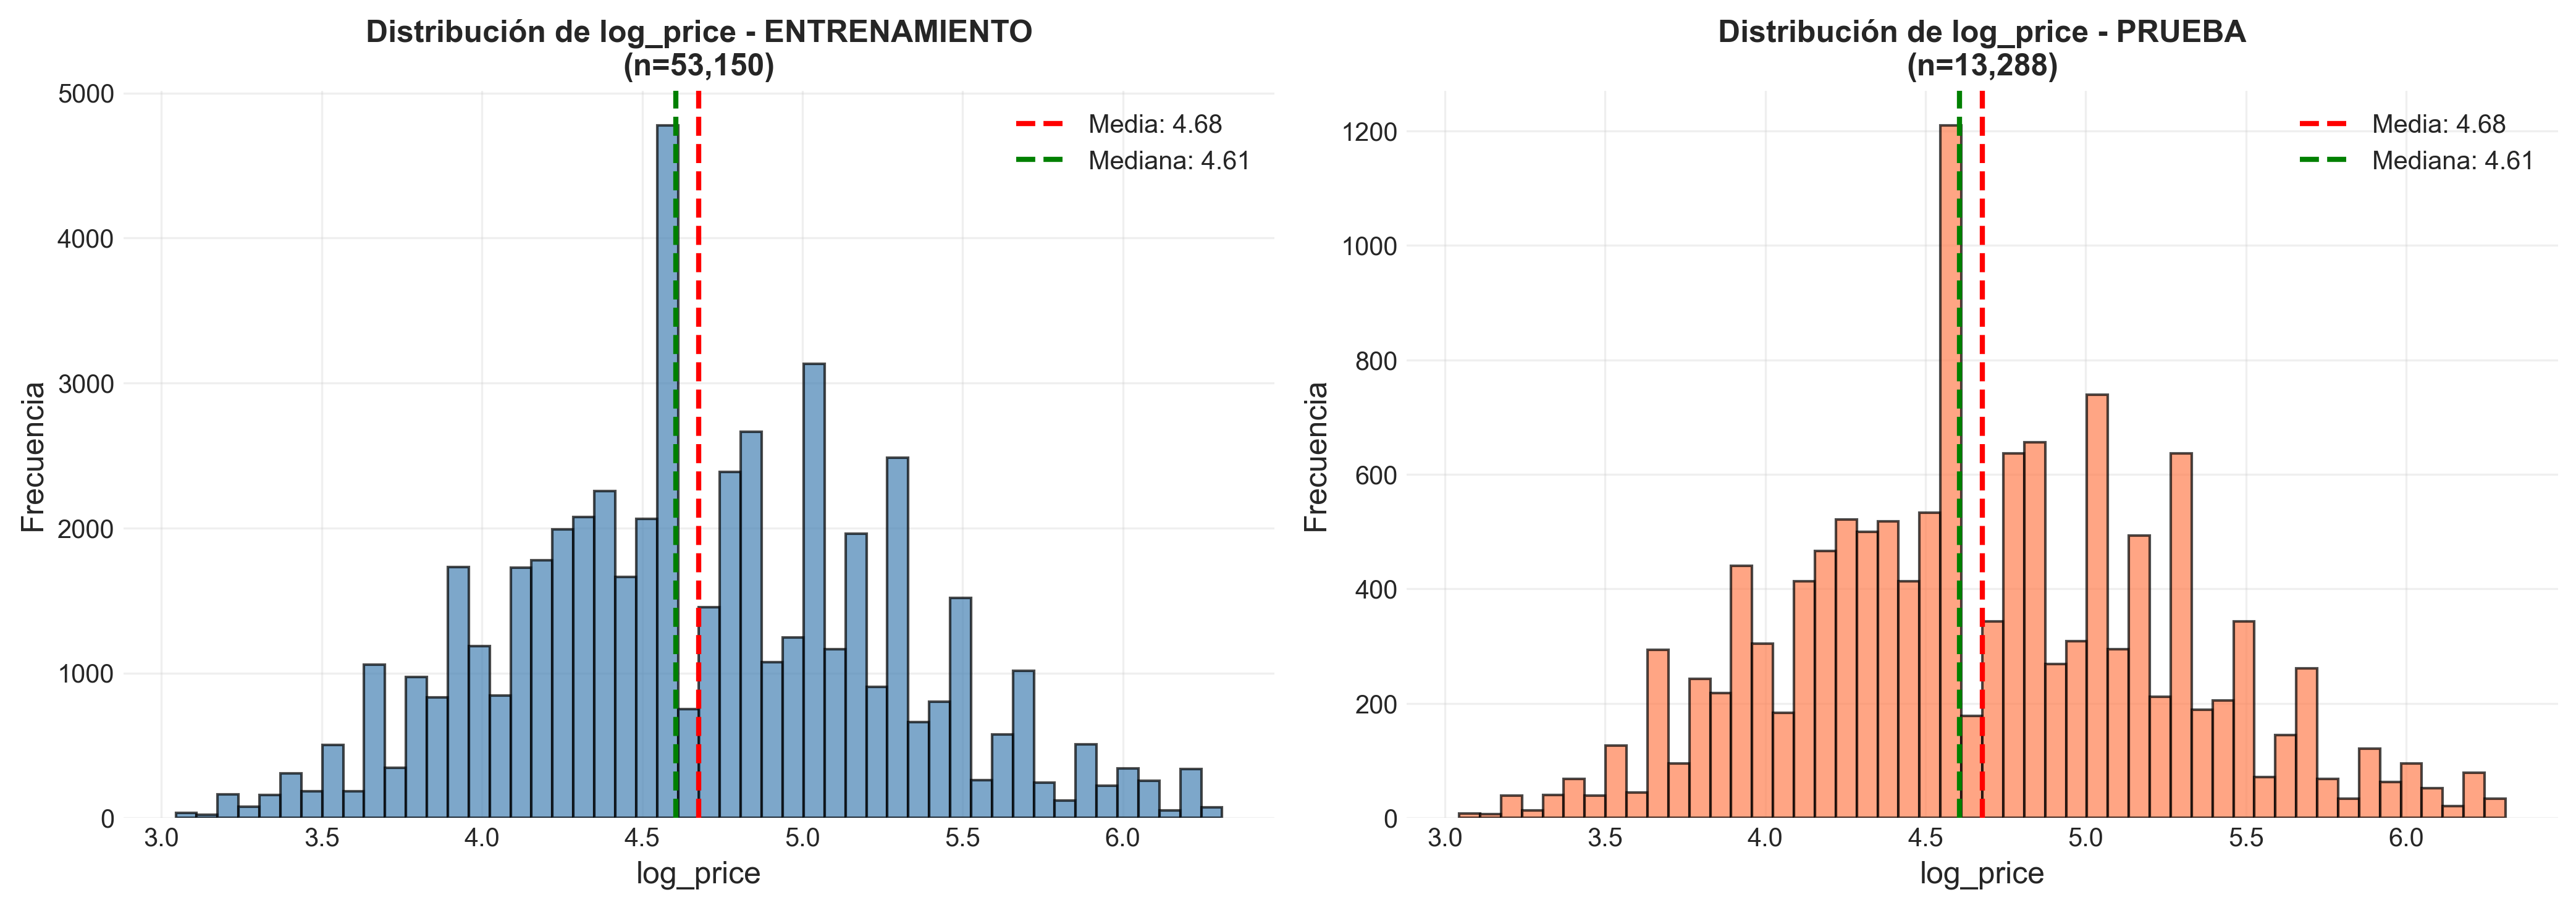
\includegraphics[width=0.95\textwidth]{../Visualizaciones/proyectoFinal/11_distribucion_train_test.png}
  \end{center}
  
  \vspace{-0.3cm}
  
  \begin{columns}
    \column{.5\textwidth}
      \textbf{Entrenamiento (80\%):}
      \begin{itemize}
        \item 53,401 observaciones
        \item Media: 4.68
        \item Desv. Est.: 0.61
      \end{itemize}
    
    \column{.5\textwidth}
      \textbf{Prueba (20\%):}
      \begin{itemize}
        \item 13,351 observaciones
        \item Media: 4.68
        \item Desv. Est.: 0.61
      \end{itemize}
  \end{columns}
  
  \vspace{0.2cm}
  
  \begin{center}
    \textbf{Random state:} 42 (reproducibilidad)
  \end{center}
\end{frame}

% ============================================
% SLIDE 7: CONSTRUCCIÓN DEL MODELO
% ============================================
\begin{frame}{6. Construcción y Entrenamiento del Modelo}
  \framesubtitle{Regresión Lineal Múltiple - Mínimos Cuadrados Ordinarios}
  
  \begin{block}{Ecuación del Modelo}
    \begin{equation*}
      \text{log\_price} = \beta_0 + \beta_1 \cdot \text{acc} + \beta_2 \cdot \text{amen} + \beta_3 \cdot \text{clean} + \sum \text{dummies}
    \end{equation*}
  \end{block}
  
  \vspace{0.3cm}
  
  \begin{center}
    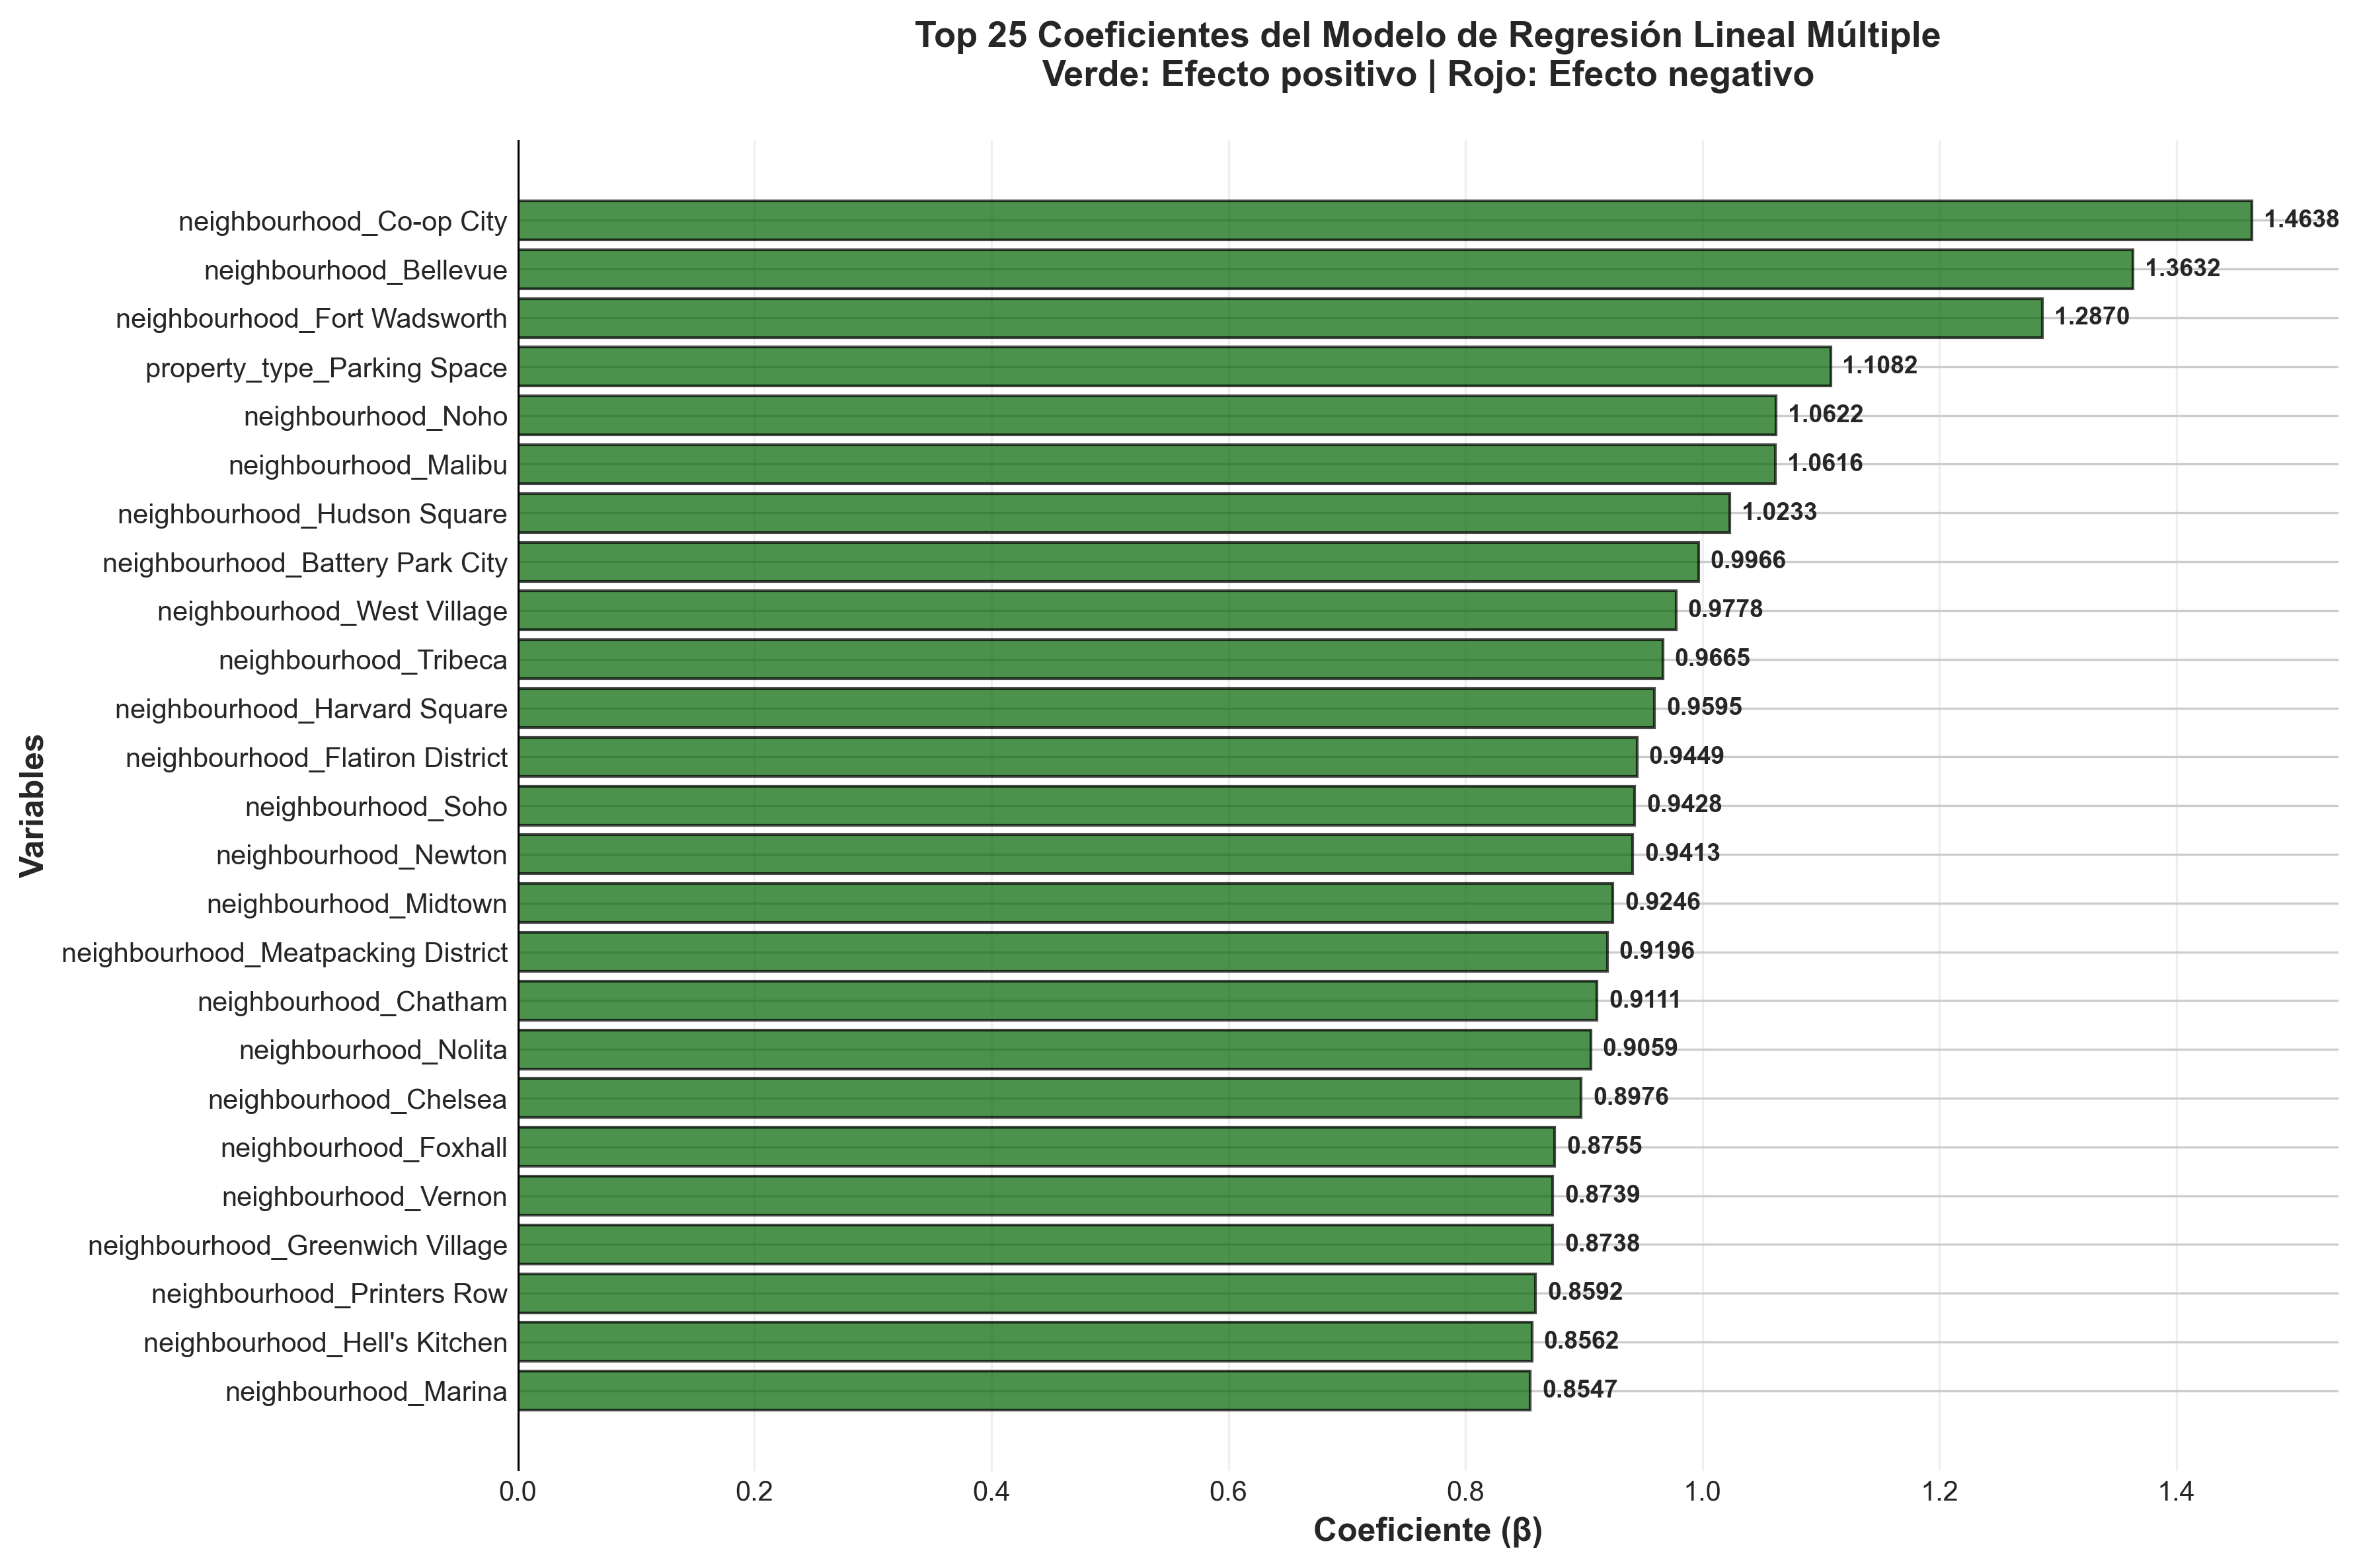
\includegraphics[width=0.75\textwidth]{../Visualizaciones/proyectoFinal/12_coeficientes_modelo.png}
  \end{center}
  
  \vspace{-0.2cm}
  
  \begin{itemize}
    \item \textbf{Método:} OLS (Ordinary Least Squares)
    \item \textbf{Variables:} 3 numéricas + room\_type + property\_type + bed\_type + neighbourhood = >650 predictores
    \item \textbf{Observaciones:} 53,401 (entrenamiento)
  \end{itemize}
\end{frame}

% ============================================
% SLIDE 8: EVALUACIÓN DEL MODELO
% ============================================
\begin{frame}{7. Evaluación del Modelo}
  \framesubtitle{Métricas de rendimiento}
  
  \begin{center}
    \begin{tabular}{lrr}
      \toprule
      \textbf{Métrica} & \textbf{Entrenamiento} & \textbf{Prueba} \\
      \midrule
      R² & 0.5993 & 0.5981 \\
      MSE & 0.1481 & 0.1483 \\
      RMSE & 0.3848 & 0.3851 \\
      MAE & 0.2921 & 0.2926 \\
      \bottomrule
    \end{tabular}
  \end{center}
  
  \vspace{0.3cm}
  
  \begin{block}{Interpretación del R²}
    El modelo explica el \alert{59.81\%} de la variabilidad en log\_price
  \end{block}
  
  \vspace{0.2cm}
  
  \begin{columns}
    \column{.5\textwidth}
      \textbf{Fortalezas:}
      \begin{itemize}
        \item[$\checkmark$] No sobreajuste
        \item[$\checkmark$] Interpretable
      \end{itemize}
    
    \column{.5\textwidth}
      \textbf{Limitaciones:}
      \begin{itemize}
        \item[$\times$] 55\% varianza no explicada
      \end{itemize}
  \end{columns}
\end{frame}

% ============================================
% SLIDE 9: P-VALUES
% ============================================
\begin{frame}{8. Significancia Estadística (P-Values)}
  \framesubtitle{Validación matemática de las variables independientes}
  
  \begin{block}{Prueba de Hipótesis}
    \begin{itemize}
      \item $\mathbf{H_0}$: La variable NO tiene efecto sobre el precio ($\beta = 0$)
      \item $\mathbf{H_1}$: La variable SÍ tiene efecto sobre el precio ($\beta \neq 0$)
      \item \textbf{Umbral de confianza:} $\alpha = 0.05$ (Nivel del 95\%)
    \end{itemize}
  \end{block}
  
  \vspace{0.2cm}
  
  \begin{columns}
    \column{.5\textwidth}
      \textbf{Resultados OLS (statsmodels):}
      \begin{itemize}
        \item \alert{Gran mayoría} de variables tienen $p < 0.05$ (Rechazamos $H_0$)
        \item Predictores base (\texttt{accommodates}, \texttt{room\_type}) muestran $p \approx 0.000$
      \end{itemize}
    
    \column{.5\textwidth}
      \begin{alertblock}{Conclusión de Significación}
        Las variables recién añadidas (\texttt{city}, \texttt{cancellation\_policy}, \texttt{instant\_bookable}) prueban ser \textbf{estadísticamente significativas} para la predicción de precios.
      \end{alertblock}
  \end{columns}
\end{frame}

% ============================================
% SLIDE 10: PREDICCIONES
% ============================================
\begin{frame}{9. Predicciones}
  \framesubtitle{Comparación valores reales vs predicciones}
  
  \begin{center}
    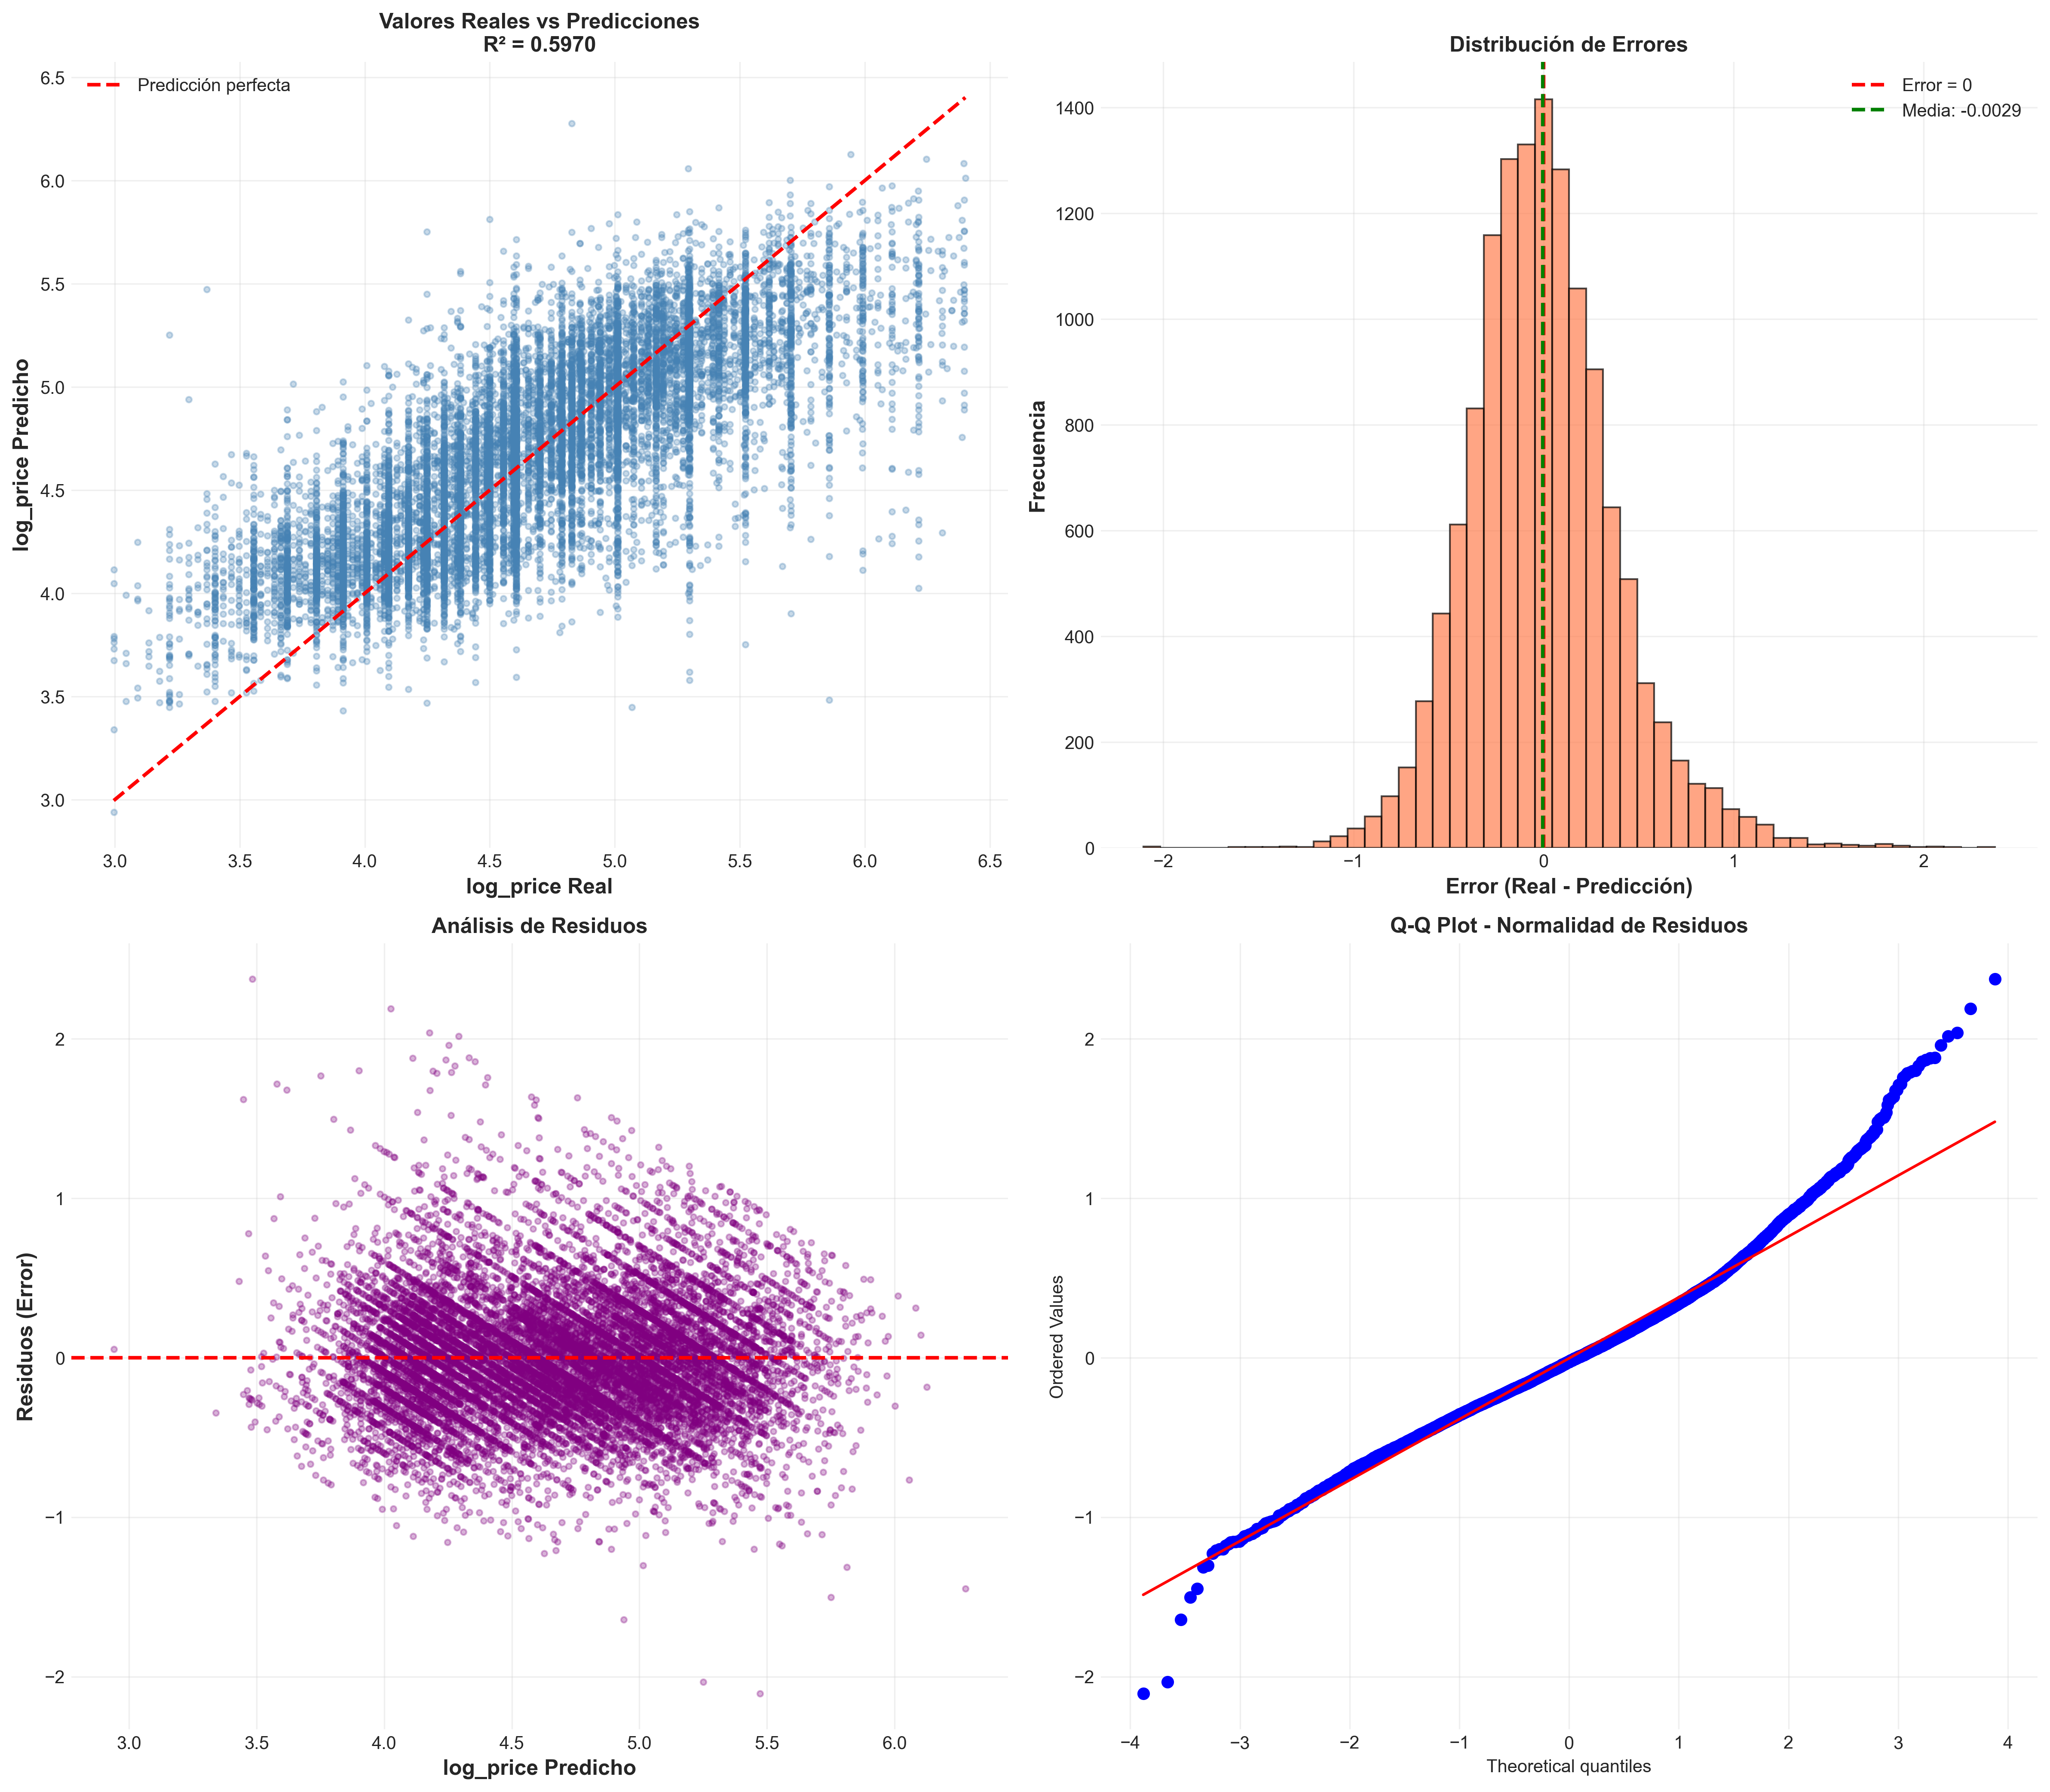
\includegraphics[width=0.95\textwidth]{../Visualizaciones/proyectoFinal/13_analisis_predicciones.png}
  \end{center}
  
  \vspace{-0.3cm}
  
  \begin{itemize}
    \item \textbf{Error medio:} -0.001 (predicciones no sesgadas)
    \item \textbf{MAE:} 0.2926 (error absoluto promedio)
    \item \textbf{Residuos:} Aproximadamente normales (Q-Q plot)
  \end{itemize}
\end{frame}

% ============================================
% SLIDE 11: MSE Y CONCLUSIONES
% ============================================
\begin{frame}{10. Error Cuadrático Medio (MSE) y Conclusiones}
  
  \begin{block}{MSE - Error Cuadrático Medio}
    \begin{itemize}
      \item \textbf{MSE Entrenamiento:} 0.1481
      \item \textbf{MSE Prueba:} 0.1483
      \item \textbf{RMSE Prueba:} 0.3851 (error promedio en escala log)
    \end{itemize}
  \end{block}
  
  \vspace{0.3cm}
  
  \begin{block}{Hallazgos Principales}
    \begin{enumerate}
      \item \textbf{Predictor principal:} accommodates (r = 0.52)
      \begin{itemize}
        \item Cada persona adicional aumenta precio $\sim$10\%
      \end{itemize}
      \item \textbf{Ubicación (neighbourhood):} Factor crítico
      \begin{itemize}
        \item 609 barrios con impactos variables en precio
        \item Mejora R² de 44\% a 60\% (+36\% explicación)
      \end{itemize}
      \item \textbf{Tipo de habitación:} También relevante
      \begin{itemize}
        \item Private room: -46\% vs Entire home
        \item Shared room: -79\% vs Entire home
      \end{itemize}
      \item \textbf{Nuevas variables integradas}
      \begin{itemize}
        \item \texttt{property\_type} y \texttt{bed\_type} (categóricas)
        \item \texttt{amenities\_count} y \texttt{cleaning\_fee} (numéricas)
      \end{itemize}
    \end{enumerate}
  \end{block}
  
  \vspace{0.2cm}
  
  \begin{alertblock}{Recomendación}
    Incorporar variables de ubicación y amenities para mejorar R²
  \end{alertblock}
\end{frame}

\end{document}
